\documentclass[11pt,a4paper,twoside]{report}

\usepackage[utf8]{inputenc}
\usepackage[T1]{fontenc}
\usepackage[head=26pt, a4paper, margin=1.2in, top=1.4in, bottom=1.75in]{geometry}
\usepackage{fancyhdr}
\usepackage{lastpage}
\usepackage[hidelinks, colorlinks, urlcolor=blue, linkcolor=black,citecolor=magenta]
{hyperref}
\usepackage{amsmath}
\usepackage{amsthm}
\usepackage{amssymb}
\usepackage{graphicx}
\usepackage{float}
\usepackage{listings}
\usepackage{tikz}
\usepackage[nottoc,numbib]{tocbibind}

% ---------------- Page and margin/header/footer Setup -----------------
\pagestyle{fancy}
%\fancyhf{} % Clears header and footer
\fancyhead{}
\fancyfoot{}
\lhead{\bfseries Calculation of homology groups\\for simplicial complexes}
\rhead{University of Copenhagen\\Computer Science}
\lfoot{Side \thepage\ af \pageref{LastPage}}
\rfoot{Nanna E. V. Bernbom}
\renewcommand{\headrulewidth}{0.4pt}
\renewcommand{\footrulewidth}{0.4pt}
% ----------------------------------------------------------------------

\newtheorem{mythm}{Theorem}[chapter]
\newtheorem{mylem}[mythm]{Lemma}
\newtheorem{mydef}[mythm]{Definition}
\newtheorem{myex}[mythm]{Example}

\newcommand\numberthis{\addtocounter{equation}{1}\tag{\theequation}}
\DeclareMathOperator{\im}{im}

\newcommand{\HRule}{\rule{\linewidth}{0.5mm}}

\begin{document}
\lstset{language=python,frame=single,breaklines=true, title=\lstname}

\begin{titlepage}
\title{\HRule \\[0.4cm]
\textbf{Calculation of Homology Groups\\for Simplicial Complexes}\\
\HRule \\[0.4cm]}
\author{\textbf{Nanna E. V. Bernbom} - zlt712\\\\
\textit{Bachelor Thesis}\\
\textit{University of Copenhagen}\\
\textit{Institute of Computer Science}\\ \\
Supervisors: Aasa Feragen and François Lauze
}
\date{June 17, 2016}

\maketitle
\thispagestyle{empty}
\end{titlepage}
\newpage\null\thispagestyle{empty}\newpage

\abstract{This report presents simplicial homology theory, a linear algebra based topological theory. The theory has been compressed into an algorithm for calculating Betti numbers, which has been implemented in \texttt{Python} using \texttt{SciPy}. The implementation and algorithm have been improved several times. It currenty has a worst case runtime of $O((m\cdot 2^n)^3)$, where $m$ is the number of maximal faces in the input, and $n$ is the maximal length of the maximal faces in the input. The runtime is dominated by the Gaussian elimination, which is part of the algorithm, and could be greatly improved by improvements to this step.

The algorithm has been implemented by use of sparse \texttt{lil\_matrix} matrices, which has greatly improved the time and space complexity of the implementation.

The program has been tested by unit testing and run on meshes, of which the biggest consisted of 12806 nodes. The tests were successful and there are no reason to doubt the correctness of the implementation. There is however an issue with the runtime of the program. It is very slow on the datasets with 26702 nodes or more, that were run as a part of the project.}

\newpage\null\thispagestyle{empty}\newpage
\tableofcontents
\newpage\null\thispagestyle{plain}\newpage
\chapter*{Introduction}
Homology theory is a part of algebraic topology and deals with holes in geometric objects. In this report, the geometric objects are simplicial complexes, which are made up of triangles of different dimensions that are glued together.

There are different types of holes. Just consider a hole in a 2-torus and compare it to the hole that is the center of a 2-sphere. Homology theory can tell the difference between different types of holes, by observing that they can be caught by spheres of different dimensions. The dimension of the $i$'th homology group is the number of holes of dimension $i$, which is what we want to know.

To find the number of holes in a geometric object is not just an interesting mathematical discipline, it also has interesting practical applications. Imagine that the simplicial complexes given to the algorithm are porous stones such as limestone, then by calculating the sizes of their homology groups one can get an insight into what their surfaces are like, and thereby get a better understanding of how to for example remove oil from limestone or store $CO_2$ in limestone. 

The reader of this report is expected to have a foundation in linear algebra, which can be brushed up in appendix \ref{ch:linalg}. It is also advisable to have an interest in topology.

Note that Gaussian elimination of big sparse matrices within reasonable time is an open problem. I have decided that this problem is outside the scope of this project.
\newpage
\section*{Workflow}
This project consists of three parts: the first being understanding simplicial homology theory, the second being to translate this theory into an algorithm which can be run on a computer, and lastly to implement this algorithm in \texttt{Python} and improve on it such that it can run on as large simplicial complexes as possible.

For the first part I read approximately half of \emph{A Short Course in Computational Geometry and Topology} by Herbert Edelsbrunner\cite{Edelsbrunner}. I did this because it seemed manageable to read a book. When I got stuck in Edelsbrunner I read some articles of which I found \emph{An Introduction to Homology} by Prerna Nadathur \cite{Nadathur} the easiest to access. For a full list of sources please look at the bibliography.

I combined the theory into the text of chapter \ref{ch:theory} where I also introduced a homemade proof of one of the central theorems of the theory (theorem \ref{thm:boundary} in this report), a definition of a Betti vector and a definition of n-simplices.

The second part is based on two blogposts by Jeremy Kun \cite{KunPrimer}\cite{Kun} but I have expanded and changed the algorithm presented in this report to fit with the API I have defined.

The third part I have preformed as an iterative process, where I first implemented a relatively naive algoritm which was somewhat mathematical in its structure. This implementation was improved several times; by use of more fitting datastructures, consideration of memory consumption and minimisation of workload. During this process I found that Gaussian elimination of big sparse martices within reasonable time is an open problem, which I have decided to be outside the scope of this project.

\chapter{Mathematical Theory} \label{ch:theory}
In this chapter, the mathematics needed to understand how to calculate homology groups is presented. For a walk-through of the linear algebra needed, please see appendix \ref{ch:linalg}.

\section{Simplicial Complexes}
Let us look at simplicial complexes. A simplicial complex consists of simplices that are 'glued' together in a nice way.

Geometrically speaking, an n-simplex is a generalisation of a triangle. It is the convex hull of $n+1$ vertices in general position \cite{Nadathur}. But since this is topology, an algebraic definition without the notion of convexity is needed.

\begin{mydef}[n-simplex]
Let $n\in\{-1,0,1,\dots\}$. An n-simplex is a structure of $n+1$ vertices containing all its subsets. In particular $\emptyset$ is the $-1$-simplex.
\end{mydef}

\begin{mydef}[faces]
Let $\Delta$ be an n-simplex. An $l$-face (or an $l$-dimensional face) of $\Delta$ is a subset of the vertices of $\Delta$ of cardinality $l+1$, it is an $l$-simplex \cite{Nadathur}. The empty set, $\emptyset$, is the unique face of dimension $-1$\cite{Allgaier}.
\end{mydef}

\begin{mydef}[maximal faces]
A face $\tau$ is said to be a maximal face if there exists no face $\delta$ such that $\tau \subsetneq \delta$ \cite[p.15]{Jonsson}.
\end{mydef}

Two simplices, $A$ and $B$, are said to be \textit{properly situated} if $A\cap B=\emptyset$ or $A\cap B = C$, where $C$ is a simplex.\cite{Nadathur}

\begin{mydef}[simplicial complexes \cite{Nadathur}]\label{def:simplicial_complexes}
A simplicial complex $\Delta$ on $[n] := \{1,2,\dots ,n\}$ is a finite set of simplices satisfying the following two conditions :
\begin{itemize}
\item For all simplices $A\in\Delta$ with $\alpha$ being a face of $A$, we have $\alpha\in\Delta$
\item $A,B\in\Delta\implies A, B $ properly situated.
\end{itemize}
\end{mydef}

A simplicial complex gives rise to a chain complex on a field $k$, in a unique way, using the following two definitions. For our purposes $k=\mathbb{R}$.

\begin{mydef}[$k^{F_i(\Delta)}$ \cite{Allgaier}]
Let $\Delta$ be a simplicial complex on $[n] := \{1,2,\dots ,n\}$. For $i\in \mathbb{Z}$, let $F_i(\Delta)$ be the set of the $i$-dimensional faces of $\Delta$ and for each $\sigma\in F_i(\Delta)$, let $e_{\sigma}$ denote the corresponding basis vector in the k-vector space, $k^{F_i(\Delta)}$. Note that for $i>n-1$ or $i<-1$, $k^{F_i(\Delta)}:=0$.
\end{mydef}

Since $k^{F_i(\Delta)}$ is a $m_i = |F_i(\Delta)|$ dimensional vector space, addition and scalar multiplication are defined on it.

For $x,y\in k^{F_i(\Delta)}$, with $x = \sum_{l=1}^{m_i}a_le_{\sigma_l}$ and $y = \sum_{l=1}^{m_i}b_le_{\sigma_l}$ where $a_l,b_l\in k$ for all $l\in\{1,2,\dots,m_i\}$, addition is defined as 
\begin{equation*}
x+y = \sum_{l=1}^{m_i}(a_l+b_l)e_{\sigma_l},
\end{equation*}
and for $x\in k^{F_i(\Delta)}$, with $x = \sum_{l=1}^{m_i}a_le_{\sigma_l}$ and $\lambda \in k$, scalar multiplication is defined as 
\begin{equation*}
\lambda x = \sum_{l=1}^{m_i}(\lambda a_l)e_{\sigma_l}.
\end{equation*}

\begin{mydef}[Boundary function \cite{Allgaier}]\label{def:boundary}
For $i=0,1,\dots,n-1$ and $\sigma\in F_i(\Delta)$, where $e_\sigma\in k^{F_i(\Delta)}$ is the corresponding basis vector, let $\partial_i: k^{F_i(\Delta)} \to k^{F_{i-1}(\Delta)}$ be given by 
\begin{equation*}
\partial_i(e_\sigma):=\sum_{j\in\sigma}\textnormal{sign}(j,\sigma)e_{\sigma\setminus j} ,
\end{equation*}
where $\textnormal{sign}(j,\sigma) = (-1)^{\textnormal{index}(j)-1}$ and $\textnormal{index}(j)$ is the index of j in $\sigma$ where the elements of $\sigma$ is listed in increasing order. For $i>n-1$ or $i\leq-1$ $\partial_i:=0$. 

The $\partial_i$'s are extended linearly to all of the $k^{F_i(\Delta)}$'s as follows: let $x = \sum_{l=1}^kg_le_{\sigma_l}\in k^{F_i(\Delta)}$ be an arbitrary chain, then $\partial_i(x)=\sum_{l=1}^kg_l\partial (e_{\sigma_l})$.
\end{mydef}
We call $\partial_i$ the $i$'th boundary function.

The chain complex is a series of vector spaces and their boundary functions as follows:
\begin{equation*}
k^{F_{n-1}(\Delta)}\overset{\partial_{n-1}}{\to}\dots\overset{\partial_{i+1}}{\to} k^{F_{i}(\Delta)}\overset{\partial_{i}}{\to}k^{F_{i-1}(\Delta)}\overset{\partial_{i-1}}{\to}\dots\overset{\partial_{0}}{\to} k^{F_{-1}(\Delta)}.
\end{equation*}

The chain complex can be expanded to an augmented chain complex as follows \cite{Allgaier}:
\begin{equation*}
0\to k^{F_{n-1}(\Delta)}\overset{\partial_{n-1}}{\to}\dots\overset{\partial_{i+1}}{\to} k^{F_{i}(\Delta)}\overset{\partial_{i}}{\to}k^{F_{i-1}(\Delta)}\overset{\partial_{i-1}}{\to}\dots\overset{\partial_{0}}{\to} k^{F_{-1}(\Delta)}\to 0.
\end{equation*}

A very important classical theorem when it comes to boundary functions is one that assert that the boundary of a boundary is the 0-object of the corresponding vector space. Among other things, this theorem embodies the concept of orientation of simplices.
\begin{mythm}\label{thm:boundary}
For all $i\in\mathbb{Z}$ 
\begin{equation*}
\partial_i\circ\partial_{i+1}=0
\end{equation*}
\end{mythm}
\begin{proof}
For $i\in\mathbb{Z}$ and $\sigma\in F_i(\Delta)$, with $e_\sigma\in k^{F_i(\Delta)}$ being the corresponding basis vector, we have 
\begin{equation*}
\partial_i(e_\sigma):=
\begin{cases}
\sum_{j\in\sigma}\textnormal{sign}(j,\sigma)e_{\sigma\setminus j} & \textnormal{ if } i=0,1,\dots,n-1 \\
0 & \textnormal{ otherwise}
\end{cases}
\end{equation*}
note that 
\begin{equation*}
0\circ\partial_{i+1}=0 \qquad \text{ and } \qquad \partial_i\circ 0 = 0.
\end{equation*}
Now let $i=0,1,\dots,n-2$. For $\sigma\in F_{i+1}(\Delta)$ we have
\begin{align*}
\partial_i(\partial_{i+1}(e_\sigma))&=\partial_i\left(\sum_{j\in\sigma}\textnormal{sign}(j,\sigma)e_{\sigma\setminus j}\right) \\
&=\sum_{j\in\sigma}\partial_i\left(\textnormal{sign}(j,\sigma)e_{\sigma\setminus j}\right)\\
&=\sum_{j\in\sigma}\textnormal{sign}(j,\sigma)\partial_i\left(e_{\sigma\setminus j}\right)\\
&=\sum_{j\in\sigma}\textnormal{sign}(j,\sigma)\sum_{k\in\sigma\setminus j}\textnormal{sign}\left(k,\sigma\setminus j\right)e_{(\sigma\setminus j)\setminus k}\numberthis \label{eq_boundary: double_sum}\\
\end{align*}
Let $a,b\in\sigma$ be arbitrarily chosen such that $a\not=b$. Then the two basis vectors $e_{(\sigma\setminus a)\setminus b}$ and $e_{(\sigma\setminus b)\setminus a}$ will appear in (\ref{eq_boundary: double_sum}). Note however, that these two basis vectors are the same, the only difference being whether $a$ or $b$ is removed first from $\sigma$. Now we can rewrite (\ref{eq_boundary: double_sum}) to
\begin{equation}
\partial_i(\partial_{i+1}(e_\sigma))=\sum_{\{j,k\}\in\sigma}\left(\textnormal{sign}(j,\sigma)\textnormal{sign}(k,\sigma\setminus j) + \textnormal{sign}(k,\sigma)\textnormal{sign}(j,\sigma\setminus k)\right)e_{\sigma\setminus\{j,k\}} \label{eq_boundary: 0}
\end{equation}
Assume without loss of generality that $\textnormal{index}(a)<\textnormal{index}(b)$. Then we have 

\begin{tabular}{l l}
\\
$\textnormal{sign}(a,\sigma) = (-1)^{\textnormal{index}(a)-1}$,  &$\textnormal{sign}(b,\sigma) = (-1)^{\textnormal{index}(b)-1}$,\\
$\textnormal{sign}(a,\sigma\setminus b) = (-1)^{\textnormal{index}(a)-1}$ and &$\textnormal{sign}(b,\sigma\setminus a) = (-1)^{(\textnormal{index}(b)-1)-1}$\\ \\
\end{tabular}
\newline
This results in
\begin{align*}
\textnormal{sign}(a,\sigma)\textnormal{sign}(b,\sigma\setminus a) &= (-1)^{\textnormal{index}(a)-1}(-1)^{(\textnormal{index}(b)-1)-1}\\
&= (-1)^{\textnormal{index}(a)-1}(-1)^{\textnormal{index}(b)-1}(-1)^{-1} \numberthis\label{eq_boundary: 1} \\
\textnormal{sign}(b,\sigma)\textnormal{sign}(a,\sigma\setminus b) &= (-1)^{\textnormal{index}(b)-1}(-1)^{\textnormal{index}(a)-1} \numberthis \label{eq_boundary: 2}\\
\end{align*}
It is clear that if (\ref{eq_boundary: 1}) is positive then (\ref{eq_boundary: 2}) will be negative, and if (\ref{eq_boundary: 1}) is negative then (\ref{eq_boundary: 2}) will be positive, so they cancel each other out when added. If we return to (\ref{eq_boundary: 0}) we see that 
\begin{equation*}
\partial_i(\partial_{i+1}(e_\sigma))=\sum_{\{j,k\}\in\sigma}0\cdot e_{\sigma\setminus\{j,k\}} 
\end{equation*}
We have now shown that $\partial_i\circ\partial_{i+1}(e_\sigma)=0$ for an arbitrary basis vector $e_\sigma$ where $\sigma\in F_i(\Delta)$. 

To finish this proof, note that for $i \in\mathbb{Z}$ by linearity of the $\partial_i$'s, for any chain \newline
$x = \sum_{l=1}^{m_i}g_le_{\sigma_l}\in k^{F_i(\Delta)}$, where $m_i=|F_i(\Delta)|$, we have 
\begin{equation*}
\partial_{i-1}(\partial_i(x)) = \partial_{i-1}\left(\partial_i\left(\sum_{l=1}^{m_i}g_le_{\sigma_l}\right)\right) = \sum_{l=1}^{m_i}g_l\partial_{i-1}(\partial_i(e_{\sigma_l}))=\sum_{l=1}^{m_i}g_l\cdot 0=0
\end{equation*}
and we are done.
\end{proof}

\section{Homology Groups}
Let $\Delta$ be an $n$-dimensional simplicial complex. Then by the previous section we have, for $i\in\{-1,0,\dots,n\}$, the set $F_i(\Delta)$ which is the set of $i$-dimensional faces of $\Delta$. To every $F_i(\Delta)$, there is a related $m_i = |F_i(\Delta)|$ dimensional vector space $k^{F_i(\Delta)}$.

Each boundary function $\partial_i:k^{F_i(\Delta)}\to k^{F_{i-1}(\Delta)}$ gives rise to two subspaces, namely the image and kernel of $\partial_i$. The image, $\im(\partial_i)$, is a subspace of $k^{F_{i-1}(\Delta)}$ and the kernel, $\ker(\partial_i)$, is a subspace of $k^{F_{i}(\Delta)}$. 

There is a relation between these image and kernel subspaces, namely that 
\begin{equation*}
\im(\partial_{i+1})\subset\ker(\partial_i).
\end{equation*}
This follows from theorem \ref{thm:boundary} in the previous section.
\begin{mylem}\label{lem:subset}
For all $i\in\mathbb{Z}$ 
\begin{equation*}
\partial_i\circ\partial_{i+1}=0 \Leftrightarrow \im(\partial_{i+1})\subset\ker(\partial_i).
\end{equation*}
\end{mylem}
\begin{proof}
Assume $\partial_i\circ\partial_{i+1}=0$ and let $a\in \im(\partial_{i+1})$, then if we take $\partial_i$ of $a$, we get that $\partial_i(a)=0\implies a\in \ker(\partial_i)$ and since $a$ was arbitrarily chosen that $\im(\partial_{i+1})\subset \ker(\partial_i)$. 

Similarly assume $\im(\partial_{i+1})\subset \ker(\partial_i)$ and let $b$ be in the pre-image of $\partial_{i+1}$ then there exists an $a\in\im(\partial_{i+1})$ such that 
$\partial_{i+1}(b)=a$ since $a\in\ker(\partial_i)$, $\partial_i\circ\partial_{i+1}=\partial_i(\partial_{i+1}(b))=0$. 
\end{proof}


For $i\in\mathbb{Z}$ the $i$'th reduced homology of $\Delta$ over $k$ can be found as the quotient space of the kernel of the $i$'th boundary function and the image of the $i+1$'th boundary function. \cite[p.2]{Allgaier}
\begin{equation}
\bar{H}_i(\Delta;k):=\ker(\partial_i)/\im(\partial_{i+1}).
\end{equation}

In the remainder of the report the word reduced will be omitted.

Having the homology groups, we can calculate their dimensions since they are vector spaces; these dimensions are called the Betti numbers of the simplicial complex. The $i$'th Betti number can be understood as the number of holes which can be caught by an $i$-sphere \cite{wikiBetti}.

What is interesting about the Betti numbers is the fact that they do not depend on the  specific simplicial complex but on the "shape" of the complex. So if two simplicial complexes represent the same object, then their Betti numbers will be the same, since the homology groups of the simplicial complexes are isomorphic to one another \cite[p. 70]{Edelsbrunner}. An example hereof can be found in the next chapter.

The dimension, $H_i$, of the $i$'th homology group can be found by the following equation \cite[p.2]{Allgaier}:
\begin{equation}\label{eq:homology_group}
H_i = \dim(\ker(\partial_i))-\dim(\im(\partial_{i+1})).
\end{equation}

Equation (\ref{eq:homology_group}) is a special case of the rank-nullity theorem\footnote{Please se theorem \ref{thm:rank_nullity} in the appendix}, with $H_i$ being the image of the mapping, $\im(\partial_{i+1})$ being the kernel and $\ker(\partial_i)$ being the source of the mapping.

A Betti vector is a way to present the Betti numbers in an orderly manner. If $H_i$ is the $i$'th Betti number, a Betti vector has the following form:
\begin{equation*}
H = (H_{-1},H_0,H_1,\dots,H_n)
\end{equation*}
where $n$ is the dimension of the simplicial complex

Like the Betti vector, an f-vector is, a way to present knowledge about a simplicial complex in a concise way. The $i$'th entry in the f-vector is the number of faces of $i$ dimensions \cite[p.15]{Jonsson}. So:
\begin{equation*}
f = (|F_{-1}|,|F_0|,\dots,|F_n|)
\end{equation*}
\chapter{Examples of Calculations of Homology Groups}
It is time for some examples on how to calculate homology groups. The details of the calculations will be spelled out for the first example, whereas the rest of the examples will be explained more briefly.
\begin{myex}
Consider the simplicial complex $\Delta_1$ in figure \ref{fig:ex1}, consisting of all the subsets of $\{1,2,3\}$, $\{2,4\},\{3,4\}$ and $\{5\}$. The example is taken from Allgaier \cite[p.2]{Allgaier}.
\begin{figure}[H]
\center
\begin{tikzpicture}
\draw [fill=gray!50] ((0,0) node[anchor = east]{1} -- (1,2) node[anchor = east]{2} -- (2,0) node[anchor = west]{3}-- (0,0);
\draw (1,2) -- (3,2) node[anchor = west]{4} -- (2,0);
\draw (4,0) node[anchor = west, circle, fill, inner sep=1pt, label = 5]{};
\end{tikzpicture}
\caption{$\Delta_1$ consists of all subsets of $\{1,2,3\},\{2,4\},\{3,4\}$ and $\{5\}$}
\label{fig:ex1}
\end{figure}
By observing $\Delta_1$ the following sets of $i$-faces, $F_i(\Delta)$, are found:
\begin{align*}
F_2(\Delta) &= \{\{1,2,3\}\}\\
F_1(\Delta) &= \{\{1,2\},\{1,3\},\{2,3\},\{2,4\},\{3,4\}\}\\
F_0(\Delta) &= \{\{1\},\{2\},\{3\},\{4\},\{5\}\}\\
F_{-1}(\Delta) &= \{\emptyset\}
\end{align*}
This results in the f-vector $f=(1,5,5,1)$ and the augmented chain complex:
\begin{equation*}
0\overset{\partial_3}{\longrightarrow} k\overset{\partial_2}{\longrightarrow} k^5\overset{\partial_1}{\longrightarrow} k^5\overset{\partial_0}{\longrightarrow} k \overset{\partial_{-1}}{\to} 0
\end{equation*}
The $\partial_i$'s are found using definition \ref{def:boundary}. 
\begin{align*}
\partial_2(e_{\{1,2,3\}})&=(-1)^0e_{\{2,3\}}+(-1)^1e_{\{1,3\}}+(-1)^2e_{\{1,2\}}\\
&=e_{\{2,3\}}-e_{\{1,3\}}+e_{\{1,2\}}\\
\partial_1(e_{\{1,2\}})&=(-1)^0e_{\{2\}}+(-1)^1e_{\{1\}}\\
&=e_{\{2\}}-e_{\{1\}}\\
\partial_1(e_{\{1,3\}})&=(-1)^0e_{\{3\}}+(-1)^1e_{\{1\}}\\
&=e_{\{3\}}-e_{\{1\}}\\
\partial_1(e_{\{2,3\}})&=(-1)^0e_{\{3\}}+(-1)^1e_{\{2\}}\\
&=e_{\{3\}}-e_{\{2\}}\\
\partial_1(e_{\{2,4\}})&=(-1)^0e_{\{4\}}+(-1)^1e_{\{2\}}\\
&=e_{\{4\}}-e_{\{2\}}\\
\partial_1(e_{\{3,4\}})&=(-1)^0e_{\{4\}}+(-1)^1e_{\{3\}}\\
&=e_{\{4\}}-e_{\{3\}}\\
\partial_0(e_{\{1\}})&=\partial_0(e_{\{2\}})=\partial_0(e_{\{3\}})=\partial_0(e_{\{4\}})=\partial_0(e_{\{5\}})=(-1)^0e_{\emptyset}\\
&=e_{\emptyset}.
\end{align*}
This results in the following matrices, describing the $\partial_i$'s with respect to the bases of $k^{F_i(\Delta)}$ and $k^{F_{i-1}(\Delta)}$
\begin{align*}
\partial_2&=
\begin{bmatrix}
1\\
-1\\
1\\
0\\
0
\end{bmatrix}\\
\partial_1&=
\begin{bmatrix}
-1 & -1 & 0 & 0 & 0\\
1 & 0 & -1 & -1 & 0\\
0 & 1 & 1 & 0 & -1\\
0 & 0 & 0 & 1 & 1\\
0 & 0 & 0 & 0 & 0
\end{bmatrix}\\
\partial_0&=
\begin{bmatrix}
1 & 1 & 1 & 1 & 1 
\end{bmatrix}
\end{align*}
The rest of the $\partial_i$'s are zero-maps.

The matrices are row reduced to find the dimensions of the images and the kernels.
\begin{align*}
\partial_2&= 
\begin{bmatrix}
1\\
-1\\
1\\
0\\
0
\end{bmatrix}
\to
\begin{bmatrix}
1\\
0\\
0\\
0\\
0
\end{bmatrix}
\end{align*}
We count $rk(\partial_2)=1$ which is another way of saying $\dim(\im(\partial_2))=1$. Now we use the rank-nullity theorem\footnote{please see theorem \ref{thm:rank_nullity} in the appendix} to calculate the dimension of the kernel of $\partial_2$.
\begin{align*}
\dim(\ker(\partial_2))&=\dim(k^{F_2(\Delta)})-\dim(\im(\partial_2))\\
&=1-1\\
&= 0
\end{align*}
We continue to row reduce $\partial_1$:
\begin{align*}
\partial_1=&
\begin{bmatrix}
-1 & -1 & 0 & 0 & 0\\
1 & 0 & -1 & -1 & 0\\
0 & 1 & 1 & 0 & -1\\
0 & 0 & 0 & 1 & 1\\
0 & 0 & 0 & 0 & 0
\end{bmatrix}
\to
\begin{bmatrix}
-1 & -1 & 0 & 0 & 0\\
0 & -1 & -1 & -1 & 0\\
0 & 1 & 1 & 0 & -1\\
0 & 0 & 0 & 1 & 1\\
0 & 0 & 0 & 0 & 0
\end{bmatrix}
\to
\begin{bmatrix}
-1 & -1 & 0 & 0 & 0\\
0 & -1 & -1 & -1 & 0\\
0 & 0 & 0 & -1 & -1\\
0 & 0 & 0 & 1 & 1\\
0 & 0 & 0 & 0 & 0
\end{bmatrix}\\
&\to
\begin{bmatrix}
-1 & -1 & 0 & 0 & 0\\
0 & -1 & -1 & -1 & 0\\
0 & 0 & 0 & -1 & -1\\
0 & 0 & 0 & 0 & 0\\
0 & 0 & 0 & 0 & 0
\end{bmatrix}
\to
\begin{bmatrix}
1 & 1 & 0 & 0 & 0\\
0 & 1 & 1 & 1 & 0\\
0 & 0 & 0 & 1 & 1\\
0 & 0 & 0 & 0 & 0\\
0 & 0 & 0 & 0 & 0
\end{bmatrix}
\end{align*}
We count $rk(\partial_1)=\dim(\im(\partial_1))=3$ and use the rank-nullity theorem to calculate the dimension of the kernel of $\partial_1$.
\begin{align*}
\dim(\ker(\partial_1))&=\dim(k^{F_1(\Delta)})-\dim(\im(\partial_1))\\
&=5-3= 2
\end{align*}
Lastly, note that 
\begin{equation*}
\partial_0=
\begin{bmatrix}
1 & 1 & 1 & 1 & 1 
\end{bmatrix}
\end{equation*}
gives us that $rk(\partial_0)=\dim(\im(\partial_0))=1$ and 
\begin{align*}
\dim(\ker(\partial_0))&=\dim(k^{F_0(\Delta)})-\dim(\im(\partial_0))\\
&=5-1= 4.
\end{align*}
Now the Betti numbers can be calculated. Remember that the $i$'th homology group is calculated as follows:
\begin{equation*}
\bar{H}_i(\Delta)=\ker(\partial_i)/\im (\partial_{i+1})\simeq k^d,
\end{equation*}
where $d$ is given by $d:=\dim(\ker(\partial_i))-\dim(\im(\partial_{i+1}))$. So 
\begin{itemize}
\item$\bar{H}_2(\Delta_1)=\ker(\partial_2)/\im(\partial_{3})=0,$
since $\dim(\ker(\partial_2))-\dim(\im(\partial_{3}))=0-0=0$,
\item$\bar{H}_1(\Delta_1)=\ker(\partial_1)/\im(\partial_{2})\simeq k,$ since $\dim(\ker(\partial_1))-\dim(\im(\partial_{2}))=2-1=1$,
\item$\bar{H}_0(\Delta_1)=\ker(\partial_0)/\im(\partial_{1})\simeq k,$
since $\dim(\ker(\partial_0))-\dim(\im(\partial_{1}))=4-3=1$, and 
\item$\bar{H}_{-1}(\Delta_1)=\ker(\partial_{-1})/\im(\partial_{0})=0,$
since $\dim(\ker(\partial_{-1}))-\dim(\im(\partial_{0}))=1-1=0$
\end{itemize}
The rest of the homology groups are 0 since they are $0/0$-expressions.
So the Betti vector is $H=(0,1,1,0)$
\end{myex}
The next example illustrates that the choice of partitioning of an object into a specific simplicial complex instead of another does not change the Betti numbers.
\begin{myex}
Consider the simplicial complex $\Delta_2$ in figure \ref{fig:ex2}, consisting of all the subsets of $\{1,2,3\},$ $\{1,3,4\},\{2,3,4\},\{2,5\},\{4,5\}$ and $\{6\}$
\begin{figure}[H]
\center
\begin{tikzpicture}
\draw [fill=gray!50] (0,0) node[anchor = east]{1} -- (1,2) node[anchor = east]{2} -- (1,1)  -- (0,0);
\draw [fill=gray!50] (0,0) -- (1,1)node[anchor = east]{3} -- (2,0) node[anchor = west]{4} -- (0,0);
\draw [fill=gray!50] (1,2) -- (1,1) -- (2,0) -- (1,2);
\draw (1,2) -- (3,2) node[anchor = west]{5} -- (2,0);
\draw (4,0) node[anchor = west, circle, fill, inner sep=1pt, label = 6]{};
\end{tikzpicture}
\caption{$\Delta_2$ consists of all subsets of $\{1,2,3\},\{1,3,4\},\{2,3,4\},\{2,5\},\{4,5\}$ and $\{6\}$}
\label{fig:ex2}
\end{figure}
By observing $\Delta_2$ the following sets of $i$-faces  $F_i(\Delta)$ are found:
\begin{align*}
F_2(\Delta) &= \{\{1,2,3\},\{1,3,4\},\{2,3,4\}\}\\
F_1(\Delta) &= \{\{1,2\},\{1,3\},\{1,4\},\{2,3\},\{2,4\},\{2,5\},\{3,4\},\{4,5\}\}\\
F_0(\Delta) &= \{\{1\},\{2\},\{3\},\{4\},\{5\},\{6\}\}\\
F_{-1}(\Delta) &= \{\emptyset\}
\end{align*}
This results in the f-vector $f=(1,6,8,3)$ and the augmented chain complex:
\begin{equation*}
0\overset{\partial_3}{\longrightarrow} k^3\overset{\partial_2}{\longrightarrow} k^8\overset{\partial_1}{\longrightarrow} k^6\overset{\partial_0}{\longrightarrow} k \overset{\partial_{-1}}{\longrightarrow} 0
\end{equation*}
The $\partial_i$'s are found using definition \ref{def:boundary}, which results in the following matrices:
\begin{align*}
\partial_2&=
\begin{bmatrix}
1 & 0 & 0 \\
-1 & 1 & 0 \\
0 & -1 & 0 \\
1 & 0 & 1 \\
0 & 0 & -1 \\
0 & 0 & 0 \\
0 & 1 & 1 \\
0 & 0 & 0 
\end{bmatrix}
\\
\partial_1&=
\begin{bmatrix}
-1 & -1 & -1 & 0 & 0 & 0 & 0 & 0 \\
1 & 0 & 0 & -1 & -1 & -1 & 0 & 0 \\
0 & 1 & 0 & 1 & 0 & 0 & -1 & 0 \\
0 & 0 & 1 & 0 & 1 & 0 & 1 & -1 \\
0 & 0 & 0 & 0 & 0 & 1 & 0 & 1 \\
0 & 0 & 0 & 0 & 0 & 0 & 0 & 0 
\end{bmatrix}
\\
\partial_0&=
\begin{bmatrix}
1 & 1 & 1 & 1 & 1 & 1 \numberthis \label{eq:ex2_0}
\end{bmatrix}
\end{align*} 
The rest of the $\partial_i$'s are zero-maps.

The matrices are row reduced to find the dimensions of the images and the kernels.
\begin{equation}\label{eq:ex2_1}
\partial_2=
\begin{bmatrix}
1 & 0 & 0 \\
-1 & 1 & 0 \\
0 & -1 & 0 \\
1 & 0 & 1 \\
0 & 0 & -1 \\
0 & 0 & 0 \\
0 & 1 & 1 \\
0 & 0 & 0 
\end{bmatrix}
\to
\begin{bmatrix}
1 & 0 & 0 \\
0 & 1 & 0 \\
0 & 0 & 1 \\
0 & 0 & 0 \\
0 & 0 & 0 \\
0 & 0 & 0 \\
0 & 0 & 0 \\
0 & 0 & 0 
\end{bmatrix}
\end{equation}
From (\ref{eq:ex2_1}) we get that $rk(\partial_2)=\dim(\im(\partial_2))=3$. By the rank-nullity theorem we calculate $\dim(\ker(\partial_2))=3-3=0$.

The same is done for $\partial_1$.
\begin{equation}\label{eq:ex2_2}
\partial_1=
\begin{bmatrix}
-1 & -1 & -1 & 0 & 0 & 0 & 0 & 0 \\
1 & 0 & 0 & -1 & -1 & -1 & 0 & 0 \\
0 & 1 & 0 & 1 & 0 & 0 & -1 & 0 \\
0 & 0 & 1 & 0 & 1 & 0 & 1 & -1 \\
0 & 0 & 0 & 0 & 0 & 1 & 0 & 1 \\
0 & 0 & 0 & 0 & 0 & 0 & 0 & 0 
\end{bmatrix}
\to
\begin{bmatrix}
1 & 0 & 0 & -1 & -1 & 0 & 0 & 1 \\
0 & 1 & 0 & 1 & 0 & 0 & -1 & 0 \\
0 & 0 & 1 & 0 & 1 & 0 & 1 & -1 \\
0 & 0 & 0 & 0 & 0 & 1 & 0 & 1 \\
0 & 0 & 0 & 0 & 0 & 0 & 0 & 0 \\
0 & 0 & 0 & 0 & 0 & 0 & 0 & 0 
\end{bmatrix}
\end{equation}
From (\ref{eq:ex2_2}) we get that $rk(\partial_1)=\dim(\im(\partial_1))=4$. Again by the rank-nullity theorem we calculate $\dim(\ker(\partial_1))=8-4=4$.

From (\ref{eq:ex2_0}) it can be seen that $rk(\partial_0)=\dim(\im(\partial_0))=1$. By the rank-nullity theorem it is calculated that $\dim(\ker(\partial_1))=6-1=5$. Now it is time for the Betti numbers.
\begin{itemize}
\item $\bar{H}_2(\Delta_2)=\ker(\partial_2)/\im(\partial_{3})=0,$
since $\dim(\ker(\partial_2))-\dim(\im(\partial_{3}))=0-0=0$,
\item$\bar{H}_1(\Delta_2)=\ker(\partial_1)/\im(\partial_{2})\simeq k,$ since $\dim(\ker(\partial_1))-\dim(\im(\partial_{2}))=4-3=1$,
\item$\bar{H}_0(\Delta_2)=\ker(\partial_0)/\im(\partial_{1})\simeq k,$
since $\dim(\ker(\partial_0))-\dim(\im(\partial_{1}))=5-4=1$, and 
\item$\bar{H}_{-1}(\Delta_2)=\ker(\partial_{-1})/\im(\partial_{0})=0,$
since $\dim(\ker(\partial_{-1}))-\dim(\im(\partial_{0}))=1-1=0$
\end{itemize}
The rest of the homology groups are 0 since they are $0/0$-expressions.
The Betti vector is then $H=(0,1,1,0)$
\end{myex}
When one compares the homology groups of $\Delta_1$ and $\Delta_2$, one sees that they are isomorphic. As it is explained in the theory section this is no coincidence, since the only difference between $\Delta_1$ and $\Delta_2$ is the partitioning into simplicies; the object which is split remains unchanged.

\chapter{Algorithm}\label{ch:algorithm}
The knowledge from the previous chapter can be compressed into the algorithm in figure \ref{fig:Algorithm} for calculating Betti vectors:
\begin{figure}[H]
\begin{lstlisting}[numbers=left]
def betti(d,maximal_faces)
    find the faces of the simplex 
    sort the faces into lengths
    for i in range(d+1) # to include bound_-1
        caluculate boundary matrix bound_i
        calculate dimensions of image and kernel of bound_i
    for i in range(d+2):
        H[i] = dim_ker_i - dim_im_i+1 # where dimensions are 0 if not calculated
    return H
\end{lstlisting}
\caption{Algorithm for calculating Betti vectors.}
\label{fig:Algorithm}
\end{figure}
This algorithm consists of several subalgorithms. We start from the beginning. To find all the faces of a simplicial complex one has to split all the maximal faces into all the smaller faces that can possibly be made from it. This method is based on definition \ref{def:simplicial_complexes} and can be found in figure \ref{fig:Algorithm_faces}
\begin{figure}[H]
\begin{lstlisting}[numbers=left]
def prepare(simplicial_complex)
    combinations = set([])
    for maximal_face in simplicial_complex:
    	sort maximal_face
        for i in range(len(maximal_face)):
            combinations.update(combinations of 0-dimensional faces in maximal_face of length i)
    return combinations    
\end{lstlisting}
\caption{Algorithm for finding faces of a simplicial complex.}
\label{fig:Algorithm_faces}
\end{figure}
To see that it makes sense to caluculate the boundary matrix partial\_i, note that the boundary functions of definition \ref{def:boundary} are linear maps from $k^{F_i(\Delta)}$ to $k^{F_{i-1}(\Delta)}$. By making all the boundary functions from $k^{F_i(\Delta)}$ to $k^{F_{i-1}(\Delta)}$, one gets a linear mapping that can be represented by a matrix, the boundary matrix. The algorithm can be found in figure \ref{fig:Algorithm_matrix}.
\begin{figure}[H]
\begin{lstlisting}[numbers=left]
def boundary(a,b):
    numrow = len(b)
    numcol = len(a)
    if numrow == 0: # if it is bound_0 being calculated
        B = matrix with 1 row and numcol columns consisting of 1s
    else:
        initialise B to a numrow*numcol matrix of 0s 
        for sigma in a:
            for j in sigma:
                i = index of sigma\j in b
                k = index of sigma in a
                B[i,k] = (-1)**(index of j in sigma) 
    return B
\end{lstlisting}
\caption{Algorithm for constructing a boundary matrix from a to b.}
\label{fig:Algorithm_matrix}
\end{figure}
How to calculate the dimensions of a matrix should be well known to the reader from linear algebra, but is included here for completeness. See figure \ref{fig:Algorithm_dims}.
\begin{figure}[H]
\begin{lstlisting}[numbers=left]
def dims(bound_i)
    perform Gausian elimination on bound_i
    im_dims = number of non-zero rows in bound_i
    ker_dims = number of rows in bound_i - im_dims
    return (im_dims, ker_dims)
\end{lstlisting}
\caption{Algorithm for finding the dimensions of the kernel and the image of a boundary matrix.}
\label{fig:Algorithm_dims}
\end{figure}
Note that Gaussian elimination until row echelon form, see figure \ref{fig:Algorithm_gauss}, has been used, instead of a faster method such as singular value decomposition because a correct result, instead of an approximation, is needed in order for the Betti values to be correct. This is also why the algorithm stops when row echelon form has been reached, instead of continuing to reduced row echelon form. The last steps from row echelon form to reduced row echelon form includes division, which can introduce round-off errors, since the matrices are integer matrices. Have a look at the discussion in the end of the report for more details.
\begin{figure}[H]
\begin{lstlisting}[numbers=left]
def elimination(bound_i)
   r,c = 0,0
   while c < number of columns and r < number of rows:
       nonzero = the nonzero row indices in [r:] of column c
       if len(nonzero) == 0:
           c += 1
           continue
       if nonzero[0]!=r:
           swap the row of r with the row of nonzero
       pivot = bound_i[r,c]
       for L in nonzero[1:]:
           temp = bound_i[L,c]
           scale row L by pivot
           subtract row r from row L, temp times
       r += 1
       c += 1
   return bound_i
\end{lstlisting}
\caption{Algorithm for Gaussian elimination.}
\label{fig:Algorithm_gauss}
\end{figure}
The last calculation in figure \ref{fig:Algorithm} is equation (\ref{eq:homology_group}).
\section{Complexity Analysis}
The algorithms can be analysed to find the worst case runtime and space complexity. 

\subsection{Dimensions of the Kernel and Image}
First of all, consider Gaussian elimination figure \ref{fig:Algorithm_gauss}. It has a worst case runtime of $O(\max(n,m)^3)$, where $n$ is the number of rows and $m$ is the number of columns. To see this, note that there are 3 places in the while loop where the worst case runtime is different from $O(1)$, which are 
\begin{itemize}
\item Finding nonzero, which takes $O(n)$.
\item Swaping two rows, which depending on the implementation takes either $O(1)$ or $O(m)$, the difference being whether it is a pointer operation or if swap copies the data.
\item The for loop, where one iteration takes $O(m)$ and there are $O(n)$ iterations resulting in a worst case runtime of $O(n\cdot m)$.
\end{itemize}
Note that the most expensive part is the for loop. Its worst case runtime now has to be multiplied by the number of times the while loop runs. That results in a runtime of $O(\min(n,m)\cdot n \cdot m)$ which can be bounded by $O(k^3)$ where $k = \max(\min(n,m), n, m)=\max(n,m)$, so the worst case runtime is $O(\max(n,m)^3)$.

The worst case space complexity of the Gaussian elimination is $O(n\cdot m)$. This can be improved by using a sparse matrix representation.

When one studies the algorithm for finding dimensions of the kernel and image of a matrix in figure \ref{fig:Algorithm_dims}, one sees that except from the Gaussian elimination the steps all take constant time, and when considering space complexity, there is nothing which takes up more space than the Gaussian elimination. Hence the time and space complexity of the algorithm is the same as Gaussian elimination.

\subsection{Making Matrices}
The algorithm for building boundary matrices found in figure \ref{fig:Algorithm_matrix} has a worst case space complexity of $O(\max(1,len(b))\cdot len(a))$, since this is the number of entries in the matrix. This number can be improved by use of sparse matrices.

The time complexity can be found as follows:
Assume it takes constant time to find the index of an element in a or b, which can be done by using dictionaries. Then the inner loop takes $O(len(\sigma))$.
The second innermost loop takes $O(len(a)\cdot len(\sigma))$.
Making a matrix of zeroes takes constant time, when the matrix is sparse, so the else branch takes $O(len(a)\cdot len(\sigma))$
The if branch takes $O(len(a))$, so the if else case takes $O(len(a)\cdot len(\sigma))$. 
For the $O(len(a)\cdot len(\sigma))$ runtime to be the worst case runtime of the algorithm it has to be slower than the construction of the previously mentioned dictionary, which is $O(len(b))$.
So the runtime is $O(\max(len(a)\cdot len(\sigma),len(b))$, which for most cases is $O(\max(len(a),len(b))$, since $len(\sigma)$ is usually small ($\leq 4$).
 

\subsection{Finding Faces}
Consider the algorithm for finding the faces of a simplicial complex, figure \ref{fig:Algorithm_faces}. If $m = len(\text{maximal faces})$ and $n = \text{maximal length of the maximal faces}$, the algorithm has a time complexity of $O(m\cdot 2^n)$. $n$ can also be found as the number of vertices of a maximal dimensional simplex in the complex, 2 for a line segment, 3 for a triangle, 4 for a tetrahedron and so forth. This results in the time complexity being $O(m)$ for the usual input. The space complexity is the same as the time complexity. The argument is as follows:
\begin{itemize}
\item For the $i$'th call to finding combinations, for $0\leq i\leq n$ , $\binom{n}{i}$ combinations are made, which also takes $O(\binom{n}{i})$ time.
\item The inner loop is run $n$ times, thereby creating $\sum_{i=0}^n\binom{n}{i}=2^n$  elements in $O(2^n)$ time.
\item The outer loop is run $m$ times thereby creating $O(2^n)$ elements per iteration resulting in $O(m\cdot 2^n)$ elements in $O(m\cdot 2^n)$ time or in $O(\text{number of faces})$ when comparing to the rest of the algorithms.
\end{itemize}

\subsection{Betti}
\begin{figure}[H]
\center
\begin{tabular}{c|c|c}
line&time&space\\
\hline
2&$O(\text{number of faces})$&$O(\text{number of faces})$\\
3&$O(\text{number of faces})$&$O(\text{number of faces})$\\
5&$O(\max(n,m))$&$O(n\cdot m)$\\
6&$O(\max(n,m)^3)$&$O(n\cdot m)$\\
8&$O(d)$&$O(d)$\\
\end{tabular}
\caption{Study of the complexity of algorithm for calculating Betti numbers, with $n=$number of rows and $m=$number of columns.}
\label{fig:runtime}
\end{figure}
When considering figure \ref{fig:Algorithm} and studying one line at a time, as done in figure \ref{fig:runtime}, one sees that the time complexity is either $O(\text{number of faces})$ or $O(k^3)$, where $k$ is the length of the maximal set of faces with a given length.

Since the number of faces is $O(\text{maximal faces})$, is just one of the considered sets when finding $k$, $O(k^3)$ is the worst case runtime of the algorithm. Note that this runtime stems from the Gaussian elimination, and if another more efficient implementation of this algorithm can be found, the entire algorithm will have a better runtime.

Considering space complexity, the algorithm has the space complexity of Gaussian elimination, since by the same argument as before $O(\text{number of rows}\cdot \text{number of columns})>O(\text{maximal faces})$.

If a worst case upper bound on the complexity of the algorithm calculating Betti numbers is to be given as an expression of the input, then the time complexity is $O((m\cdot 2^n)^3)$, where $m$ is the number of maximal faces, and $n$ is the maximal length of the maximal faces. The space complexity will then be $O((m\cdot 2^n)^2)$.

\chapter{Implementation}
As part of this project, the algorithm to calculate Betti vectors, described in chapter \ref{ch:algorithm}, has been implemented in python as the program \texttt{Betti}. In order to use OFF files as input, another program \texttt{Preproc}, which pre-processes the OFF file to a format that \texttt{Betti} can read, has been made. It also turned out to be necessary to translate \texttt{MATLAB} matrices into a format \texttt{Betti} can read. This resulted in an expansion of \texttt{Preproc} in the form of \texttt{preproc\_m.py}.
The entire source code can be found in appendix \ref{ch:source_code} or on GitHub: \url{https://github.com/Bernbom/Betti}

\begin{figure}[H]
\center
\begin{tikzpicture}
	\node[fill = lightgray,shape=rectangle,draw=black] (preproc) at (0,-1) {preproc};
	\node[fill = lightgray,shape=rectangle,draw=black] (betti) at (3,-1) {betti};
	\node[fill = lightgray,shape=rectangle,draw=black] (bettifile) at (6,-1) {betti\_file};
	
	\node[fill = lightgray,shape=rectangle,draw=black] (preprocM) at (0,0) {preproc\_m};
	
	\node[fill = lightgray,shape=rectangle,draw=black] (hom) at (3,1) {hom};
	\node[shape=rectangle,draw=black] (homTest) at (5,1) {hom\_test};
			
	\node[fill = lightgray,shape=rectangle,draw=black] (bound) at (-2,3) {bound};
	\node[shape=rectangle,draw=black] (boundTest) at (0,3) {bound\_test};	
	\node[fill = lightgray,shape=rectangle,draw=black] (gauss) at (2,3) {gauss};
	\node[shape=rectangle,draw=black] (gaussTest) at (4,3) {gauss\_test};
	\node[fill = lightgray,shape=rectangle,draw=black] (imKer) at (6,3) {im\_ker};
	\node[fill = lightgray,shape=rectangle,draw=black] (prep) at (8,3) {prep};
	
	\node[fill = lightgray,shape=rectangle,draw=black] (row) at (2,5) {row};
	\node[shape=rectangle,draw=black] (rowTest) at (4,5) {row\_test};	
	
	\path[->](row) edge (gauss);
	\path[->](row) edge (rowTest);
	\path[->](gauss) edge (gaussTest);
	\path[->](bound) edge (boundTest);
	\path[->](bound) edge (hom);
	\path[->](gauss) edge (hom);
	\path[->](imKer) edge (hom);
	\path[->](prep) edge (hom);
	\path[->](hom) edge (betti);
	\path[->](hom) edge (bettifile);
	\path[->](hom) edge (homTest);
\end{tikzpicture}
\caption{The call structure of the programs}
\label{fig:program_structure}
\end{figure}
Figure \ref{fig:program_structure} shows how the different files in the implementation call one another. 

\section{Dependencies}\label{ch:dependencies}
\texttt{Betti} and \texttt{Preproc} were made on a computer running Ubuntu 16.04 LTS with 4 GB RAM running Python 2.7.11+ with SciPy version 0.17.0 and NumPy version 1.11.0. Furthermore, the \texttt{SciPy} submodule scipy.sparse has been used throughout \texttt{Betti}.

The programs have been tested on a computer running Ubuntu 14.04 LTS with 16 GB RAM running Python 2.7.6 with SciPy version 0.17.1 and NumPy version 1.8.2.

\section{How to Call the Program} \label{ch:how2call}
The main function in \texttt{Betti} is \texttt{hom.betti} which can either be imported into a python source file and be run from there or one can call the file \texttt{betti.py} from the terminal as in figure \ref{fig:bettipseudo},
\begin{figure}[H]
\begin{lstlisting}[language=bash]
$ python betti.py <d> <maximal faces> 
\end{lstlisting}
\caption{How to call \texttt{Betti} using \texttt{betti.py}}
\label{fig:bettipseudo}
\end{figure}
where \texttt{<d>} is an integer which is the dimensions of the simplicial complex, and \texttt{<maximal faces>} is a string listing the maximal faces of the simplicial complex being investigated\footnote{Note that the string \texttt{<maximal faces>} can contain more faces than the maximal ones, but only needs the maximal ones. This is a property \texttt{betti\_file.py} takes advantage of.}. The maximal faces are represented as a comma-separated string. A zero dimensional face can be represented by any symbol combination except blanc spaces, i.e. tab, space, newline, ect., comma, or the symbol chosen to indicate the start and end of a string usually ' or ". A higher dimensional face consists of combinations of zero dimensional simplices separated by commas.

Figure \ref{fig:betti} is an example of how the function is used:
\begin{figure}[H]
\begin{lstlisting}[language=bash]
$ python betti.py 2 '1,2,3 2,4 3,4 5'
[0,1,1,0] 
\end{lstlisting}
\caption{Example of how to call \texttt{Betti} using \texttt{betti.py} }
\label{fig:betti}
\end{figure}

\texttt{Betti} can also be called by calling \texttt{betti\_file.py} from the terminal as in figure \ref{fig:bettifile}.
\begin{figure}[H]
\begin{lstlisting}[language=bash]
$ python betti_file.py <d> <file containing maximal faces> 
\end{lstlisting}
\caption{How to call \texttt{Betti} using \texttt{betti\_file.py}}
\label{fig:bettifile}
\end{figure}
Note that the second argument in figure \ref{fig:bettifile} must have the faces of the complex in one line split by spaces and each face split into zero dimensional faces by commas as seen in figure \ref{fig:betti}. An OFF file can be made into this format using the program \texttt{Preproc} as seen in figure \ref{fig:preproc}. The terminal will write "success" upon a successful run of \texttt{preproc}.

\begin{figure}[H]
\begin{lstlisting}[language=bash]
$ python preproc.py <OFF file> <output file> 
\end{lstlisting}
\caption{How to call \texttt{Preproc} from the terminal.}
\label{fig:preproc}
\end{figure}

It is also possible to translate a file containing a simplicial complex, with one maximal face per line split into 0-faces by tabs, into the right format for \texttt{Betti} using \texttt{preproc\_m.py}. The mentioned file format can be made by making a mesh in \texttt{MATLAB} using \texttt{DistMesh} and the copying the \texttt{t}-matrix into an empty file.

\begin{figure}[H]
\begin{lstlisting}[language=bash]
$ python preproc_m.py <simplicial complex file> <output file> 
\end{lstlisting}
\caption{How to call \texttt{preproc\_m} from the terminal.}
\label{fig:preproc_m}
\end{figure}

\section{Description of the Implementation}
As mentioned, the primary function in \texttt{Betti} is the \texttt{hom.betti} function. It is the function which calculates the Betti vector of the \texttt{d} dimensional simplicial complex. \texttt{hom.betti} is given the integer \texttt{d} as first argument and a string containing the maximal faces as second argument. The limitations to the naming of the simplices can be found in section \ref{ch:how2call}. 

As can be seen from figure \ref{fig:program_structure}, \texttt{hom.betti} uses the functions in the files \texttt{bound.py}, \texttt{gauss.py}, \texttt{im\_ker.py} and \texttt{prep.py}. They are \texttt{bound.boundary}, \texttt{gauss.elimination}, \texttt{im\_ker.dims} and \texttt{prep.prepare}. \texttt{gauss.elimination} calls the functions of \texttt{row} which are \texttt{row.swap}, \texttt{row.scale} and \texttt{row.combine}.

\subsection{Modules Used}
The two modules \texttt{NumPy} and \texttt{SciPy} and their submodules have been used throughout the code for representation of matrices. The primary matrix representation has been the sparse \texttt{lil\_matrix} in the \texttt{scipy.sparse} module but the regular matrix type from \texttt{NumPy} has been used in one case to make a matrix that was then changed to a sparse matrix right away. 

The module \texttt{Itertools} has been used in the function \texttt{prep.prepare}, which takes a string of the maximum simplices of a simplicial complex and returns a list of all the simplices in the simplicial complex. \texttt{Itertools} has been used to create the strings representing the simplices. The source code can be found in appendix \ref{ch:source_code}.

The module \texttt{sys} has been used in \texttt{betti.py}, \texttt{betti\_file.py}, \texttt{preproc.py} and \newline \texttt{preproc\_m.py} for making the main functions.

\subsection{The Functions}

This section goes through all the functions and describes how they work.

\begin{description}
\item[\texttt{preproc.simcom\_prep(off\_file, target\_file)}:] given an OFF file containing a simplicial complex returns a file containing the simplicial complex in one line in a format ready for \texttt{betti\_file.py}. 
\item[\texttt{preproc\_m.simcom\_prep(input\_file, target\_file)}:] given a file containing a simplicial complex, with one maximal face per line split into 0-faces by tabs, returns a file containing the simplicial complex in one line, in a format ready for \texttt{betti\_file.py}.
\item[\texttt{hom.betti(d,<maximal faces>)}:] calculates the Betti vector of the \texttt{d} dimensional simplicial complex with the given maximal faces.
\item[\texttt{prep.prepare(<maximal faces>)}:] given the maximal faces of a simplicial complex, as a string, creates a list of faces in that complex.
\item[\texttt{bound.boundary(a,b)}:]creates the boundary matrix from a to b, where a and b are given as lists of strings. The boundary matrix contains the coefficients of the boundary functions: $\partial(e_{\sigma}) = \sum_i((-1)^{index(i)}e_{\sigma\setminus i})$.
\item[\texttt{gauss.elimination(A)}:] given a matrix A returns the Gaussian eliminated matrix.
\item[\texttt{im\_ker.dim(A)}:] given a matrix from \texttt{gauss.elimination} returns the dimensions of its image and kernel.
\item[\texttt{row.swap(A,i,j)}:] in matrix A: swap row i and j.
\item[\texttt{row.scale(A,i,n)}:] in matrix A: multiply row i with n.
\item[\texttt{row.combine(A,i,j,n)}:] in matrix A: add row j to row i n times.
\end{description}
Furthermore, there are the main functions \texttt{betti.py} and \texttt{betti\_file.py} described in section \ref{ch:how2call}.

\subsection{Optimisations}
Some optimisations have been made in order to make it possible to run the programs with big datasets\footnote{Big here means more than a million nodes if one ignores the Gaussian elimination. If one is interested in running the entire program the maximum dataset which has been run is with 600000 nodes.}.
\begin{description}
\item[The Betti algorithm] Instead of using the mathematical most intuitive algorithm where all the boundary matrices are calculated first after which all the dimensions are calculated followed by the Betti numbers, an algorithm where only one matrix is needed at a time in the RAM has been used. This results in the program being able to handle larger inputs without running out of RAM.
\item[Type of matrices] Another way of minimising the use of memory in the program is to use a sparse matrix representation, which only represent the non-zero entries of the matrices and ignores the zero entries. In this version of the program, the built-in \texttt{SciPy} sparse matrix representation \texttt{lil\_matrix} has been used. An argument for this choice is presented in the concluding remarks.
\item[Use of dictionary] Instead of making a linear index search for faces in b in \texttt{bound.boundary} a dictionary has been used to contain the faces in b, where the key is the tuple equvalent to the face and the value is the index of the face in b.
\item[Use of sets] In \texttt{prep.prepare}, when making the list of faces, a set was used to contain the finished faces. This resulted in only new faces being added to the set, which decreased the use of memory in the function.
\item[Use of \texttt{xrange}] The method \texttt{xrange} has been used instead of \texttt{range} throughout the program where it made sense. That is where the iterator contained more than a few elements. This optimisation results in a smaller memory usage.
\item[The Gaussian elimination algorithm] In \texttt{gauss.elimination}, different optimisations have been used. First and foremost, the sparse structure of the input matrix has been utilised. This is done by only considering the rows that are nonzero in column $j$. Furthermore, the algorithm only iterates through the rows that are further down in the matrix than the current row. This results in fewer calls to the row utility functions of \texttt{row.py}. 

For correctness the algorithm has also been changed from the regular Gaussian elimination, that continues until reduced row echelon form is reached, to one that stops when row echelon form has been reached. This improvement eliminates the risk of introducing round-off errors during the scaling step of the algorithm.
\item[Use of \texttt{getrowview}] In \texttt{row.py} the matrix operations are as inplace as possible. A major contribution to this is the use of \texttt{getrowview} which is a built-in method of \texttt{scipy.sparse.lil\_matrix}, which instead of copying the given row merely returns a view of the given row. 
\item[Finding the dimensions of image and kernel] When finding the dimensions of the image and kernel, \texttt{im\_ker.dims} makes use of the built-in \texttt{lil\_matrix} method \texttt{nonzero}. This is instead of counting the nonzero rows manually.
\end{description}
\subsubsection{Unsuccessful optimisations}
There are also some optimisations that did not work. These are optimisations that tried to avoid using Gaussian elimination. This was done due to the fact that Gaussian elimination has a worst case runtime of $O(n^3)$ (please see chapter \ref{ch:algorithm}) and after all the other optimisations, the Gaussian elimination was clearly the slowest section of the algorithm.

What is common for the methods experimented with, is that they try to estimate the rank of the boundary matrices instead of calculating the exact rank. This turned out to be a bad idea, since all the tests ended up failing with the estimating methods by giving the wrong results and when the methods were tried on the biggest dataset described in section \ref{ch:test_data}, the result was a memory error. 

The methods experimented with were LU decomposition, SVD, QR and a built-in \texttt{SciPy} method called \texttt{estimate\_rank}.

My best guess to why the methods gave the wrong result is that the boundary matrices are rank deficient. I have found sources saying that at least SVD \cite{wikiSVD} has problems with rank deficient matrices. Furthermore the boundary matrices contain only $-1$'s, 0's and 1's in the beginning, and since the mentioned methods are iterative I can imagine some problems with the numbers being so close to one another.
\section{Tests}
As shown in figure \ref{fig:program_structure}, there are four files which test the implementation of \texttt{Betti}. These are \texttt{hom\_test.py}, \texttt{bound\_test.py}, \texttt{gauss\_test.py} and \texttt{row\_test.py}, the primary test being \texttt{hom\_test.py}. It tests whether the entire program returns the correct Betti vector on a given simplicial complex. It has 7 test cases testing both simplicial comlexes of 2 and 3 dimensions, simplicial complexes given in diffenrent orders, simplicial complexes with long 0-face names, and the two corner cases of an empty simplicial complex and a simplicial complex containing only a 0-simplex. 

The two files \texttt{gauss\_test.py} and \texttt{bound\_test.py}, test the implementation of the two second most important functions of the program.

The file \texttt{row\_test.py} contains one test per function in \texttt{row.py} to test that the utility functions behave as expected.

The rest of the implementation has been tested using manual testing during the development. All the tests have been successful on the current version of \texttt{Betti}.

The four files containing tests have been made using the unittest Python module. They can be called from the terminal as seen in figure \ref{fig:how2test}:
\begin{figure}[H]
\begin{lstlisting}[language=bash]
$ python <test file name>
\end{lstlisting}
\caption{How to call a test.}
\label{fig:how2test}
\end{figure}
Upon a succesful run of a test, the terminal will print "Ran <n> tests in <s>s OK" where <n> is th number of tests, and <s> is the number of seconds it took to run the tests.

\section{Run on Datasets}\label{ch:test_data}
Three datasets made with \texttt{DistMesh} in \texttt{MATLAB} have been run on the program. See figure \ref{fig:mesh_oneHole}, \ref{fig:mesh_torus} and \ref{fig:mesh_sphere} for visualisations. The datasets were copied from \texttt{MATLAB} into a file and then translated to the right format using \texttt{preproc\_m.py}. 
\begin{figure}[H]
\center
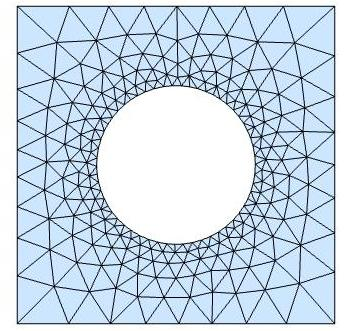
\includegraphics[scale=0.5]{oneComponentOneHole.jpg}
\caption{Test dataset with one component and one hole.}
\label{fig:mesh_oneHole}
\end{figure}
The dataset of figure \ref{fig:mesh_oneHole} gave the Betti vector $[0,0,1,0]$ as expected. The torus of figure \ref{fig:mesh_torus} also gave the expected result: $[0,0,2,1,0]$, together with the sphere of figure \ref{fig:mesh_sphere} which gave the Betti vector: $[0,0,0,1,0]$.
\begin{figure}[H]
\begin{minipage}[b]{0.45\linewidth}
\center
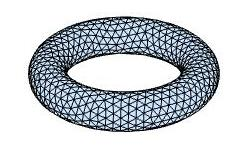
\includegraphics[scale=0.5]{torus.jpg}
\caption{Test dataset which is a torus.}
\label{fig:mesh_torus}
\end{minipage}
\hspace{0.5cm}
\begin{minipage}[b]{0.45\linewidth}
\center
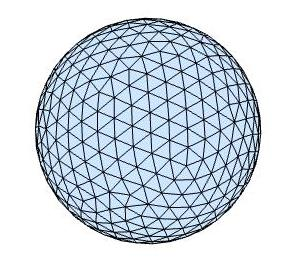
\includegraphics[scale=0.5]{sphere.jpg}
\caption{Test dataset which is a sphere.}
\label{fig:mesh_sphere}
\end{minipage}
\end{figure}
The following datasets have been run using \texttt{preproc.py} and \texttt{betti\_file.py} on the big computer described in section \ref{ch:dependencies}. All the datasets are meshes described by OFF files. 

The triangulation of a teapot shown in figure \ref{fig:teapot} has been run by \texttt{Betti}. It is a mesh consisting of 12806 nodes. The result, which came in less than an hour, was the following Betti vector $[0,3,38,0,0]$. Which means that there are 4 conected components and 38 tunnels in the data.
\begin{figure}[H]
\begin{minipage}[b]{0.45\linewidth}
\center
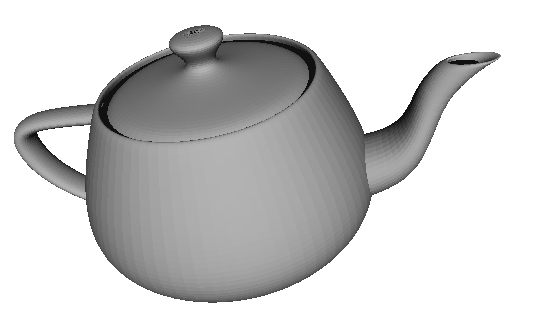
\includegraphics[scale=0.5]{teapot00.png}
\end{minipage}
\hspace{0.5cm}
\begin{minipage}[b]{0.45\linewidth}
\center
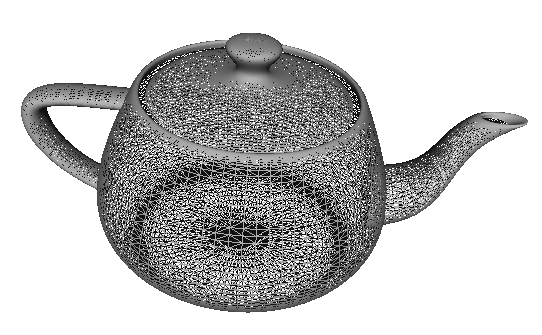
\includegraphics[scale=0.5]{teapot01.png}
\end{minipage}
\caption{A triangulation of a teapot}
\label{fig:teapot}
\end{figure}
This result may look a bit strange, but not as strange as one might think. When one studies the mesh of the teapot, one sees that it consists of 4 parts: a lid, a spout, a handle and a body. Concerning the tunnels it is clear that there are at least one tunnel through the handel, one through the spout. This is a total of two holes. The rest of the holes most likely come from the fact, that the teapot is not a simplicial mesh, but a mesh used in computer graphics. This can result in the triangles of the triangulation having more corners than three, thereby ending up as holes. 

There is no reason to doubt the correctness of \texttt{Betti}, since all the tests including the runs on the simple meshes have returned the desired results.

\texttt{Betti} has also run on 3 other datasets of different sizes with varied success. 
The datasets are 3D network structures of some biological data to which voluminous meshes have been fitted.
\begin{figure}[H]
\center
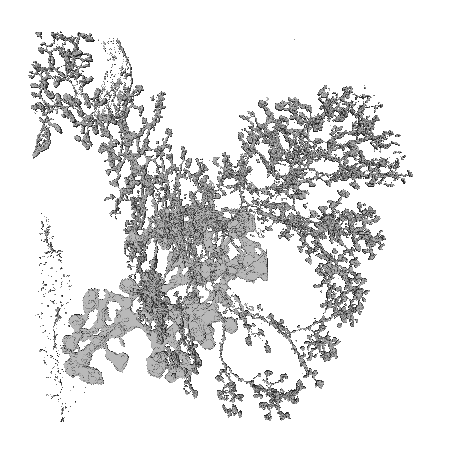
\includegraphics[scale=0.5]{downsampled00.png}
\caption{The biggest dataset}
\label{fig:mesh_down}
\end{figure}
The first dataset, see figure \ref{fig:mesh_down}, is a mesh with 1088346 nodes. Based on the fact that it takes 5 minutes for \texttt{Betti} to calculate 1 column in the second Gaussian elimination, I guess it will take approximately a year for \texttt{Betti} to run the data, since I have calculated that there are approximately 4-5 million columns in the second boundary matrix of the dataset. This is based on the fact of there being approximately 2000000 triangles in the dataset and the columns of the second boundary matrix are equivalent to the edges of the dataset.

When one ignores the Gaussian elimination, it takes 10-15 minutes for \texttt{Betti} to run the dataset on the big computer described in section \ref{ch:dependencies}. There are no problems with the memory, as long as it is run on the mentioned computer. On the smaller computer, it takes a lot longer to run the program and it runs out of memory before it is done.
\begin{figure}[H]
\center
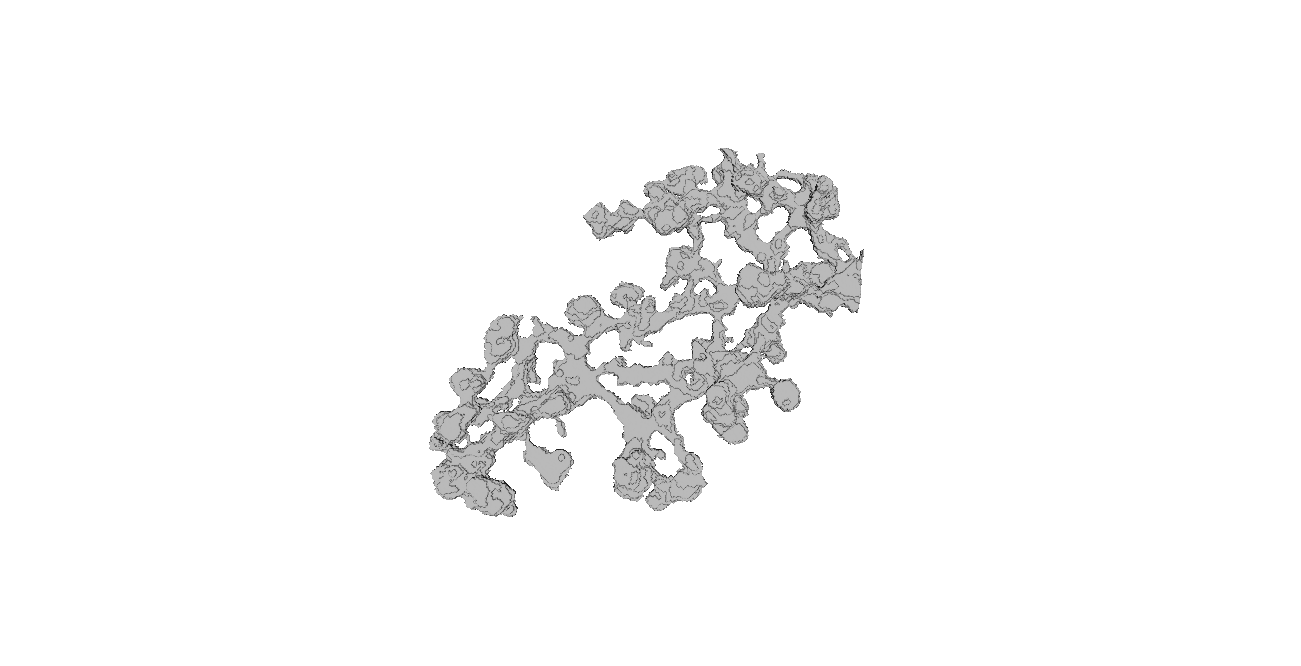
\includegraphics[scale=0.5]{testmesh2d00.png}
\caption{The second biggest dataset}
\label{fig:mesh_2d}
\end{figure}
The mesh of figure \ref{fig:mesh_2d} was run on a older incorrect version of the program. It took 15 days to run the program, so there is not time to run it and get a correct Betti vector before the defence of this project. The mesh has 214271 nodes.

\begin{figure}[H]
\center
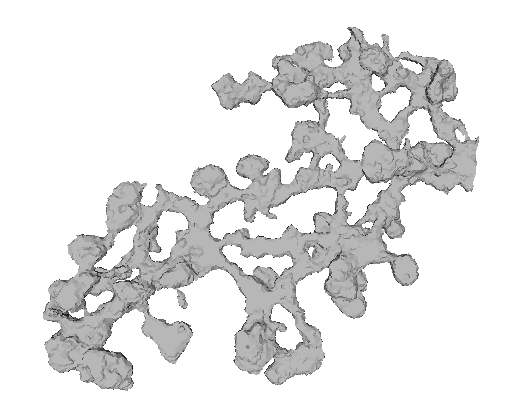
\includegraphics[scale=0.5]{testmesh00.png}
\caption{The smallest dataset}
\label{fig:mesh_}
\end{figure}
The dataset visualised in figure \ref{fig:mesh_} was run in approximately six and a half hours, on an older version of \texttt{Betti}. It is a mesh with 26702 nodes. The result of the run was the following Betti vector $[0,40,36410,0,0]$. These Betti numbers were estimated to be to high, and resulted in several bugs being found in the code. When the dataset is run on the newest, correct version of \texttt{Betti}, the runtime is much slower, and it has not been possible to get a result, before the deadline of this report. It is most likely an increase in the number of nonzero elements in the matrix, and thereby the number of calculations, that is to blame for the increased runtime.

\chapter{Concluding Remarks}
In this report, the basics of simplicial homology have been presented, including the definition of homology groups of a simplicial complex and the associated Betti numbers.
A more abstract view point would expand it to singular homology theory, though not necessary here, for the determination of Betti numbers.

The algorithm for calculating Betti numbers, presented in this report, has a worst case time complexity of $O((m\cdot 2^n)^3)$, and a space complexity of $O((m\cdot 2^n)^2)$. Here $m$ is the number of maximal faces, and $n$ is the maximal length of the maximal faces. $n$ can also be found as the number of vertices of a maximum dimensional simplex in the complex - 2 for a line segment, 3 for a triangle, 4 for a tetrahedron ect. So for a reasonable input, this is at most the dimension of the imbedding space +1. The actual complexities are therefore $O(m^3)$ for time and $O(m^2)$ for space. 

Both of the complexities are loose and worst case, but it is difficult to make them tighter. When one looks at the space complexity, the actual complexity is dependent of the sparseness of the boundary matrices. Since it is difficult to to say anything about the sparseness of the boundary matrices during the Gaussian elimination, a more tight bound is difficult to give. The time complexity is again dependent of the Gaussian eliminations, and the sparseness of the boundary matrices during these eliminations. 

It is desireable to be able to run the program on datasets with more than a million nodes. This will make it possible to use it for characterising porous stones, as mentioned in the introduction. Even though the actual complexity of the program is most likely between $O(m^3)$ and $O(m^2)$, it has to go down to somewhere between $O(m^2)$ and $O(m)$, in order for the program to be able to run on such big datasets.

Several experiments have been made in the quest for improving the complexities of the Betti number calculating program implemented as part of this project. The program is implemented in \texttt{Python} and is called \texttt{Betti}. Some of the experiments were successful, others were not. Of the successful experiments one can mention to use a sparse matrix representation called \texttt{lil\_matrix}. 

A \texttt{lil\_matrix} is saved in the memory as two arrays of arrays containing respectively the indices and the nonzero elements of the matrix\cite{csr}. This representation makes it easy to find the elements of the matrix row by row, but not too expensive to find them column by column, plus it is possible to change the sparsity structure of the matrix relativly inexpensively. Another advantage of \texttt{lil\_matrix} is its method called \texttt{getrowview} which returns a pointer to the given row without copying it. \texttt{lil\_matrix} was choosen instead of the to two representatioins called \texttt{dok\_matrix} and \texttt{csr\_matrix}. These two formats are respectively a dictionary over the nonzero elements\cite{wikiSparse} and three arrays where one contains all the nonzero data of the matrix, one contains all the column indices of the nonzero elements and the last contains the indices of the row starts in the column array\cite{karlrupp}.

Just like \texttt{lil\_matrix} the two other matrix representations have advantages and disadvantages. The \texttt{dok\_matrix} is efficient when looking up individual elements, because of the dictonary structure, and is efficient - even more than the \texttt{lil\_matrix} - when it comes to changes to the sparsity structure. Its disadvantages is that it does not have an efficient way to look up a row, but has to go through the dictionary for every element. It is also lacking the \texttt{getrowview} method of \texttt{lil\_matrix}\cite{dok}. 

The \texttt{csr\_matrix} is very efficient when it comes to looking up a row, but is inefficient when it comes to changes to the sparsity structure, and is very inefficient when it comes to looking up columns\cite{csr}.

The documentation of \texttt{SciPy.sparse} is very sparse, so it is difficult to say whether \texttt{lil\_matrix} is the right matrix representation for this project. Since both row and column look-ups are needed in the Gaussian elimination I assesed it to be the best representation of the ones available.

Other improvements made to the implementation includes use of dictionaries and sets, minimisation of data needed in the memory at a time, by only having one matrix in the memory at a time, and minimisation of work done in the Gaussian elimination by only bringing the matrix to row echelon form.

During the project, experiments were made to avoid Gaussian elimination. These included, but was not limited to, experiments with SVD and LU elimination, but none of the methods tried gave good results. If they could run on the input data they gave wrong results.

The program has been tested two different ways. The first method was unit testing which has been done throughout the development. In the last phase of the development, the program was also run on meshes, to test the usability of the program. The biggest mesh, with a successful run, consisted of 12806 nodes.  In this phase a program called \texttt{Preproc} was made to translate the meshes into a format accepted by \texttt{Betti}. The tests that finished were run without problems, but the runtime of \texttt{Betti} resulted in only approximately half the tests finishing before the deadline of this report.

In the future this project can be expanded to solve problems with persistent homology, please see \cite{Edelsbrunner} for a definition. 

Another possible future improvement to the project would be to improve the Gaussian elimination. This could be done by implementing some bookkeeping concerning which coordinates of the matrix that are nonzero, in a way that makes it easy to find the elements that are nonzero both from a row and from a column approach.



\begin{thebibliography}{9}

\bibitem{Allgaier} Allgaier et al., \emph{Homology of Simplicial Complexes}, 2004
\bibitem{Edelsbrunner}
Herbert Edelsbrunner, \emph{A Short Course in Computational Geometry and Topology}, Springer, 2014
\bibitem{Jonsson} Jakob Jonsson, \emph{Introduction to simplicial homology}, February 3, 2011
\bibitem{KunPrimer} Jeremy Kun, \emph{Homology Theory a Primer}, \url{http://jeremykun.com/2013/04/03/homology-theory-a-primer/}
\bibitem{Kun} Jeremy Kun, \emph{Computing Homology}, \url{http://jeremykun.com/2013/04/10/computing-homology/}
\bibitem{Nadathur} Prerna Nadathur, \emph{An Introduction to Homology}, August 16, 2007
\bibitem{LinAlg} Niels V. Pedersen, \emph{Liniær Algebra}, 2nd edition, Københavns Universitet Matematisk Afdeling, 2009
\bibitem{karlrupp} Karl Rupp, \emph{Sparse Matrix Transposition: Datastructure Performance Comparison} \url{https://www.karlrupp.net/2016/02/sparse-matrix-transposition-datastructure-performance-comparison/}
\bibitem{csr} unknown, \emph{csr\_matrix}, \url{https://github.com/scipy/scipy/blob/v0.17.1/scipy/sparse/csr.py#L21-L437}, Scipy source code
\bibitem{dok} unknown, \emph{dok\_matrix}, \url{http://docs.scipy.org/doc/scipy-0.14.0/reference/generated/scipy.sparse.dok_matrix.html}, Scipy dokumentation
\bibitem{wikiBetti} unknown, \emph{Betti Number}, \url{https://en.wikipedia.org/wiki/Betti_number}, Wikipedia, March 29 2016
\bibitem{wikiSparse} unkown, \emph{Sparse Matrix}, \url{https://en.wikipedia.org/wiki/Sparse_matrix}, Wikipedia, June 11 2016
\bibitem{wikiSVD} unknown, \emph{SVD}, \url{https://en.wikipedia.org/wiki/Singular_value_decomposition}, Wikiperia, June 8 2016
\bibitem{wikiQuo} unknown, \emph{Quotient Space (linear algebra)}, \url{https://en.wikipedia.org/wiki/Quotient_space_(linear_algebra)}, Wikipedia, March 25 2016
\end{thebibliography}
\newpage\null\newpage
\appendix
\chapter{Linear Algebra}\label{ch:linalg}
In this section the linear algebra that is used when homology groups are calculated are presented. This section is primarily based on Niels V. Pedersen's book \emph{Lineær Algebra} \cite{LinAlg}.
\section{Vector Spaces, Subspaces and Quotient Spaces}
Let $V$ be a set, and $k$ a field. For $V$ to be a vector field over $k$, two operations, namely scalar product and sum, must be defined which live up to 8 rules as described by Pedersen \cite[pp. 85-86]{LinAlg}. It is included here for completeness.
\begin{mydef} 
Let $V$ be a set and $k$ a field. $V$ is a vector space over $k$ if for $x,y\in V$ and $\lambda\in k$ the scalar product $\lambda x\in V$ and the vector sum $x+y\in V$ and for arbitrary vectors $x,y,z\in V$ and scalars $\lambda,\mu\in k$ the following rules are fulfilled:
\begin{enumerate}
\item $(x+y)+z = x+(y+z)$
\item $x+0=x$
\item $x+(-x)=0$
\item $x+y=y+x$
\item $\lambda(x+y)=\lambda x+\lambda y$
\item $(\lambda+\mu)x=\lambda x + \mu x$
\item $(\lambda\mu)x=\lambda(\mu x)$
\item $1x=x$
\end{enumerate}
\end{mydef}
Having a vector space $V$, it is possible to define a subspace $U$ of $V$.\cite[p.93]{LinAlg}
\begin{mydef}
A non-empty subset $U\subset V$ is called a subspace if the following conditions hold
\begin{enumerate}
\item if $x\in U$ and $\lambda\in k$ then $\lambda x\in U$
\item if $x,y\in U$ then $x+y\in U$
\end{enumerate} 
\end{mydef}
Now it is time to define a quotient space. In order to do that, an equivalence relation is needed. 

Let $V$ be a vector space over a field $k$ and $U\subset V$. We say $a\sim b$ if and only if $a-b\in U$. It is clear that all elements of $U$ are equivalent.
This equivalence relation gives rise to a set of equivalence classes $[x]=\{x+u,u\in U\}$
The quotient space $V/\sim = V/U$ is then defined as this set of equivalence classes over $V$ by $\sim$.
One can define scalar multiplication and addition on the quotient space in the following way. \cite{wikiQuo}
\begin{itemize}
\item $\lambda[x]=[\lambda x]$, for all $\lambda\in k$
\item $[x]+[y]=[x+y]$
\end{itemize}
To see that the first definition is well defined, let $x'\in[x]$ be arbitrarily chosen. Then $x'$ can be written as $x'=x+u$ for some $u\in U$ and 
\begin{equation*}
\lambda x' = \lambda (x + u) = \lambda x + \lambda u \in [\lambda x],
\end{equation*}
since $\lambda u \in U$ by the definition of a subspace.

Similarly can it be proven that the second definition is well defined. Let $x'\in[x]$ and $y'\in [y]$ be arbitrarily chosen. Then $x'$ can be written as $x'=x+u$ for some $u\in U$ and $y' = y+u'$ for some $u'\in U$. It is now clear that
\begin{equation*}
x'+y'=(x+u)+(y+u')=x+y+(u+u')\in [x+y],
\end{equation*}
since $u+u'\in U$ by the definition of a subspace.


\section{The Rank-Nullity Theorem}
The Rank-Nullity Theorem is used throughout the entire project, since it is an easy way to calculate the dimensions of the kernel of mappings such as the boundary maps. The theorem is as follows \cite[p. 109]{LinAlg}: 
\begin{mythm}\label{thm:rank_nullity}
Let $f:U\to V$ be a linear mapping then the following holds
\begin{equation*}
\textnormal{rk}f+\dim(\ker)=\dim U
\end{equation*}
\end{mythm}

To finish this section, remember that the rank of a linear map does not change when it is row reduced.

\chapter{Source Code}\label{ch:source_code}
In this appendix the entire code made during the project can be found.
\section{Betti}
\lstinputlisting{../code/betti.py}
\lstinputlisting{../code/betti_file.py}
\newpage
\lstinputlisting{../code/hom.py}
\newpage
\lstinputlisting{../code/prep.py}
\lstinputlisting{../code/bound.py}
\lstinputlisting{../code/gauss.py}
\lstinputlisting{../code/row.py}
\newpage
\lstinputlisting{../code/im_ker.py}
\subsection{Tests}
\lstinputlisting{../code/hom_test.py}
\lstinputlisting{../code/bound_test.py}
\lstinputlisting{../code/gauss_test.py}
\newpage
\lstinputlisting{../code/row_test.py}
\newpage
\section{Preproc}
\lstinputlisting{../code/preproc.py}
\lstinputlisting{../code/preproc_m.py}
\end{document}
